\documentclass[tikz,border=5mm,12pt]{standalone}

\begin{document}
  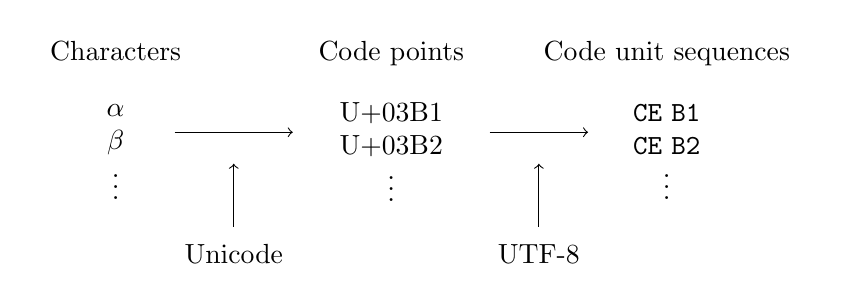
\begin{tikzpicture}
    \node[text width=20mm,align=center] at (0,0) {Characters\strut};
    \node[text centered,text width=20mm] at (0,-12.5mm) {
      $\alpha$ \\
      $\beta$ \\
      $\vdots$};

    \node[text width=25mm,align=center] at (35mm,0) {Code points\strut};
    \node[text centered,text width=20mm] at (35mm,-12.5mm) {
      U+03B1 \\
      U+03B2 \\
      $\vdots$};

    \node[text width=40mm,align=center] at (70mm,0) {Code unit sequences\strut};
    \node[text width=40mm,align=center] at (70mm,-12.5mm) {
      \texttt{CE B1} \\
      \texttt{CE B2} \\
      $\vdots$};

    \draw[->] (7.5mm,-10mm) -- (22.5mm,-10mm) coordinate[midway] (C1);
    \draw[->] (47.5mm,-10mm) -- (60mm,-10mm) coordinate[midway] (C2);

    \draw[<-] (C1)+(0,-4mm) -- ++(0,-12mm) node[anchor=north,yshift=-1mm] {Unicode};
    \draw[<-] (C2)+(0,-4mm) -- ++(0,-12mm) node[anchor=north,yshift=-1mm] {UTF-8};
  \end{tikzpicture}
\end{document}
